\chapter{Архитектура системы и технологии}
\label{chap:architecture}

\section{Общая архитектура}

Система состоит из нескольких компонентов:

\begin{enumerate}
    \item storage — база данных MongoDB \cite{chodorow2010mongodb}, в которой хранятся все необходимые для работы данные;
    \item indexer — инструмент для индексации репозитория;
    \item backend — веб-сервер, который реализует всю логику составления ответа на запросы клиента;
    \item router — веб-сервер, задача которого заключается в раздачи статики (файлов frontend) и проксировании запросов к бекенду.
    \item frontend — клиентская часть, обеспечивающая клиенту доступ к данным. 
\end{enumerate}

Их взаимодействие можно изобразить следующим образом:

\begin{figure}[H]
    \centering
    \includesvg[height=12\baselineskip]{figures/architecture.svg}
    \caption{Взаимодействие компонентов}
\end{figure}

Для развертывания серверной части (компонентов storage, backend, router) применяется технология контейнеризации Docker \cite{dockerbook}. К этим компонентам предоставляются \texttt{Dockerfile}, а также файл \texttt{docker-compose.yml}, облегчающий запуск сервисов. Собранный таким router будет также отдавать собранные файлы frontend.

Хотя indexer также предоставляет Dockerfile, описывающий сборку этого компонента, но реализация механизмов его запуска возлагается на пользователя. Это связано с тем, что не существует универсального способа узнавать об изменениях в Git-репозитории и имеет смысл внедрить индексацию репозитория в существующие процессы CI/CD. Соответствующая документация находится в директории компонента.

В качестве основного языка программирования для этого проекта был выбран Rust из-за его удобства и инструментов для написания производительного кода \cite{trpl}.

В качестве веб-сервера для проксирования запросов и раздачи статики используется Caddy \cite{Caddy}, позволяющий легко описать всю конфигурацию, а также, при необходимости, обеспечить поддержку HTTP/2 и TLS.

\section{Структура проекта}

Проект организован следующим образом:
\begin{itemize}
    \item \texttt{backend/}
        \begin{itemize}
            \item \texttt{mongo-model} — специальный процедурный макрос, облегчающий описание типов моделей и взаимодействие с ними в базе данных.
            \item \texttt{shatterbird-cli} — вспомогательная программа, реализующая некоторый отладочный и демонстрационный функционал.
            \item \texttt{shatterbird-indexer} — программа, загружающая данные об индексируемом репозитории в хранилище.
            \item \texttt{shatterbird-server} — программа, запускающая веб-сервер, отвечающий на запросы клиента.
            \item \texttt{shatterbird-storage} — библиотека, содержащая описание модели данных и предоставляющая некоторые функции для доступа к базе данных. 
            \item \texttt{shatterbird-utils} — библиотека, содержащая общий функционал.
            \item \texttt{Dockerfile} — файл, описывающий сборку серверной части и всех инструментов.
        \end{itemize}
    \item \texttt{frontend/} — проект, описывающий сборку кастомизированного дистрибутива Visual Studio Code \cite{vscode}, а также содержащий расширения для взаимодействия с серверной частью. В том числе, содержит следующие файлы:
        \begin{itemize}
            \item \texttt{Caddyfile} — файл, описывающий конфигурацию Caddy.
            \item \texttt{Dockerfile} — файл, описывающий сборку пользовательской части и запуск Caddy.
            \item описание файлов реализации пользовательской части приведено в разделе \ref{section:frontend-impl}.
        \end{itemize}
    \item \texttt{docker-compose.yml} — файл, описывающий порядок сборки и запуска всего сервиса
\end{itemize}

Полный список файлов проекта возможно найти в приложении \fullref{addendum:repo}.

\section{Модель данных}
\label{section:data-model}

Данные хранятся в документ-ориентированной базе данных MongoDB. Каждый объект описан на языке Rust и автоматически сериализуется в совместимый с MongoDB формат BSON с помощью библиотеки serde \cite{serde-rs}. 

Для описания модели данных применяется специальный тип \texttt{Id<T>}, который является оберткой вокруг стандартного типа \texttt{ObjectID} из MongoDB, но добавляет информацию о том, какому именно типу объекта принадлежит тот или иной идентификатор (эта информация не сохраняется при сериализации).

Также, чтобы облегчить создание моделей и уменьшить количество ошибок, реализован специальный процедурный макрос, который на этапе компиляции позволяет убедиться в том, что каждый тип модели имеет имя коллекции, а также предоставляет поле \texttt{id} типа \texttt{Id<Self>} (то есть, собственный идентификатор), которое используется в качестве уникального идентифкатора в MongoDB.

В приложении \fullref{addendum:models} приводятся описания объектов с использованием синтаксиса языка TypeScript, что достаточно близко отражает, то, как они хранятся в базе данных.

При этом для обеспечения эффективного доступа к данным, в базе данных строятся следующие индексы:

\begin{itemize}
    \item В коллекции \texttt{nodes} для поля \texttt{oid}, содержащего хэш-сумму объекта в Git-репозитории.
    \item В коллекции \texttt{ranges} для поля \texttt{line\_id}, чтобы быстро находить все подстроки, находящиеся внутри той или иной строки. Их число в одной строке обычно невелико и для нахождения нужной дополнительные индексы не требуются.
    \item В коллекции \texttt{edges} строится составной индекс на полях \texttt{edge} (содержит тип ребра) и \texttt{out\_v} (содержит идентифкатор вершины, из который выходит это ребро). Такой индекс позволяет эффективно находить исходящие из данной вершины рёбра определённого типа, что является важнейшим шагом алгоритма вычисления ответа.
    \item В коллекции \texttt{vertices} строится частичный индекс на поле \texttt{data.range}, содержащее идентифкатор объекта Range для тех вершин графа, которые представляют подстроки в LSIF. Этот индекс строится только на тех вершинах, которые имеют \texttt{data.vertex} равным «\texttt{Range}».
    \item Дополнительно в коллекции \texttt{vertices} строится индекс на поле \texttt{data.vertex}, содержащее тип той или иной вершины.
\end{itemize}

\section{Взаимодействие клиентской части и серверной}
\label{section:api}

В этом разделе описываются маршруты API, предоставляемые серверной частью. Все методы (за исключением \texttt{/fs/blobs/:id}) здесь возвращают свой ответ с помощью JSON и используют коды ошибок 404, 400 и 500 для обозначения, соответственно, ситуаций когда объект не был найден, запрос был некорректен или произошла внутренняя ошибка сервера.

Поверхность API также разделить на две части: предоставляющую доступ к файлам и предоставляющую обработчики запросов LSP-клиента.

Во-первых, рассмотрим доступ к файлам. Большинство методов здесь возвращают объект \texttt{FullNode}, аналогичный хранимому в базе данных объекту \texttt{Node}, но обогащенный дополнительной информацией, которая почти всегда будет необходима клиенту. Это позволяет уменьшить количество запросов к серверу и улучшить отзывчивость приложения. Описание объекта представлено в приложении \fullref{models:fullnode}.

Ниже приведен список методов:

\begin{itemize}
    \item \texttt{GET /fs/commits} — возвращает информацию обо всех проиндексированных коммитах (возвращает объект \texttt{Commit});
    \item \texttt{GET /fs/commits/by-id/:commit} — возвращает информацию об отдельном коммите по его идентификатору в хранилище (возвращает объект \texttt{Commit});
    \item \texttt{GET /fs/commits/by-oid/:oid} — возвращает информацию об отдельном коммите по его идентификатору в Git-репозитории (возвращает объект \texttt{Commit});
    \item \texttt{GET /fs/tree/:commit} — возвращает корневую директорию коммита (возвращает объект \texttt{FullNode});
    \item \texttt{GET /fs/tree/:commit/*uri}, где uri содержит путь к файлу — возвращает информацию об узле, находящемся по указанному пути (возвращает объект \texttt{FullNode});
    \item \texttt{GET /fs/nodes/:id} — возвращает узел файлового дерева по его идентифкатору в базе данных (возвращает объект \texttt{FullNode});
    \item \texttt{GET /fs/blobs/:id} — возвращает содержимое указанного бинарного файла (как поток байт).
\end{itemize}

Затем рассмотрим взаимодействие LSP-клиента с сервером. Стоит отметить, что протокол LSP \cite{languageserver} предполагает использование двустороннего канала связи и определяет взаимодействие клиента и сервера с помощью JSON-RPC \cite{jsonrpc} следующим образом:

\begin{minted}{text}
-> {"jsonrpc": "2.0", "id": 1,
    "method": "textDocument/hover", "params": { ... }}
<- {"jsonrpc": "2.0", "id": 1, "result": { ... }}
\end{minted}

Однако в случае этого проекта нет смысла в наличии двустороннего канала, поскольку состояние индексов можно считать неизменным и таким образом сервер никогда не будет отправлять сообщения клиенту. Поэтому в проекте вместо JSON-RPC применяются обычные HTTP-запросы следующим образом (второстепенные заголовки опущены):
\begin{itemize}
    \item Запрос:
    \begin{minted}[gobble=4]{text}
    POST /lsp/textDocument/hover
    Content-Type: application/json
    
    { ... } // содержимое "params" из jsonrpc-запроса
    \end{minted}
    
    \item Ответ:
    \begin{minted}[gobble=4]{text}
    Content-Type: application/json
    
    { ... } // содержимое "result" из jsonrpc-ответа
    \end{minted}
\end{itemize}

Здесь в запросе используется POST, поскольку запросы имеют тело, однако при этом запросы являются идемпотентными и не меняют какого-либо состояния в хранилище.

Благодаря поддержке протокола HTTP/2 \cite{rfc9113} сервером, клиент не инициализирует новое TCP-подключению для каждого запроса, а переиспользует единственное ранее установленное для разных запросов. В том числе HTTP/2 позволяет в рамках этого подключения делать новые запросы даже до завершения предыдущих. Это позволяет сохранять отзывчивость, сравнимую с обычным JSON-RPC.

Сервер возвращает код ошибки 400 в случае некорректного запроса, код ошибки 404, если запрос относится к несуществующему файлу и код ошибки 500 в случае непредвиденных ошибок сервера. Гарантируется, что на любой запрос корректного LSP-клиента сервер отвечает кодом 200. В частности, это означает, что даже если ответ пустой (например, определение символа не было найдено), то сервер ответит кодом 200 с пустым ответом, в соответствии с оригинальной спецификацией протокола LSP \cite{languageserver}. 

Реализованы следующие методы:

\begin{itemize}
    \item \texttt{POST /lsp/initialize} — Cервер отвечает информацией о том, какие возможности протокола LSP он поддерживает. А именно, заявляет о поддержке методов «\texttt{textDocument/hover}», «\texttt{textDocument/definition}» и «\texttt{textDocument/references}».
    \item \texttt{POST /lsp/textDocument/hover} — Сервер отдает содержимое всплывающего окна рядом с курсором, которое должно появляться при наведении на тот или иной символ.
    \item \texttt{POST /lsp/textDocument/definition} — Сервер находит определение символа под курсором и возвращает его местоположение.
    \item \texttt{POST /lsp/textDocument/references} — Сервер находит все использования символа под курсором и возвращает список местоположений.
\end{itemize}

Типы объектов, передающихся в телах запросов и ответов, полностью соответствуют спецификации LSP \cite{languageserver} для соответствующих методов и здесь не приводятся.

Описание алгоритма поиска ответа приведено в разделе \fullref{lsp-algorithm}.

Сам же сервер собирается в единственный статически слинкованный исполняемый файл (как большинство программ на языке Rust) и для запуска требует указать в параметрах командной строки строку подключения к базе данных и адрес, на котором сервер будет принимать запросы. Для облегчения запуска приложения из контейнера, допускается указать приложению файл, который будет содержать дополнительные параметры командной строки.

\section{Реализация клиентской части}
\label{section:frontend-impl}

Клиентская часть представляет собой сборку Visual Studio Code, модифицированную таким образом, чтобы использовалась реализация клиента LSP, совместимая с сервером, и виртуальная файловая система. При этом она должна работать в браузере пользователя без необходимости дополнительных действий.

Результат сборки сайта имеет следующую структуру:
\begin{itemize}
    \item \texttt{/index.html} — точка входа, загружающая Visual Studio Code и описывающая местоположение всех необходимых для её работы файлов.
    \item \texttt{/vscode-web/…} — в директории \texttt{vscode-web} содержатся файлы, обеспечивающие работу Visual Studio Code.
    \item \texttt{/product.json} — файл \texttt{product.json} описывает конфигурацию этой сборки Visual Studio Code: её название и список дополнительных расширений. Среди прочего, этот файл оказывает дополнительно загрузить следующее расширение:
    \item \texttt{/shatterbird/} — директория содержит расширение, обеспечивающие интеграцию с сервером.
    \item \texttt{/shatterbird/manifest.json} — каждое расширение должно содержать файл, описывающий необходимые для его загрузки параметры. В частности, этот файл указывает, что код расширения находится в файле \texttt{extension.js}.
    \item \texttt{/shatterbird/extension.js} — этот файл содержит модуль, выполняющий инициализацию и запуск расширения. Он генерируется из исходных кодов во время сборки.
\end{itemize}

Само же расширение состоит из двух частей.

Во-первых, расширение предоставляет реализацию виртуальной файловой системой, используя данные с сервера для отображения файлов и директорий. Файловая система доступна только для чтения, редактор не позволяет вносить в них изменения. В рамках реализации интерфейса \texttt{FileSystemProvider} были предоставлены следующие методы:
\begin{itemize}
    \item \texttt{stat(uri: Uri): FileStat} — возвращает информацию об узле файловой системы: является ли тот файлом или директорией, а также его размер. Всегда сообщает, что файл доступен только для чтения.
    \item \texttt{readDirectory(uri: Uri): [string, FileType][]} — возвращает список дочерних узлов директории, а также для каждого сообщает его тип (файл или директория).
    \item \texttt{readFile(uri: Uri): Uint8Array} — возвращает содержимое файла в виде массива байт. Если файл является текстовым, то собирает его из отдельных строк и возвращает результат.
\end{itemize}

Также все полученные с сервера узлы файлового дерева кэшируются в памяти, чтобы улучшить отзывчивость. При этом важно отметить, что Visual Studio Code не запрашивает данные для тех узлов дерева, которые не отображаются пользователю, поэтому нет необходимости выкачивать всё файловое дерево репозитория, что позволяет быстро начинать просмотр даже больших проектов.

Во-вторых, расширение реализует провайдер для Language Server. Для этого реализованы три класса:
\begin{itemize}
    \item \texttt{LanguageClient extends BaseLanguageClient} — класс инициализирует подключение к серверу и настраивает его использование для всех файлов, находящихся на виртуальной файловой системе, а также конфигурирует транспорт для передачи сообщений (а именно, Reader и Writer).
    \item \texttt{Reader extends AbstractMessageReader} — класс, который передает в Visual Studio Code в совместимом формате ответы от сервера после их получения. Здесь происходит конвертация ответов сервера в сообщения JSON-RPC.
    \item \texttt{Writer extends AbstractMessageWriter} — реализует отправку сообщений на сервер в совместимом формате, то есть сообщения-запросы JSON-RPC превращаются в http-запроса. Причем впоследствии ответ сервера передается в Reader для дальнейшего отображения пользователю.
\end{itemize}

Для написания расширения был выбран язык программирования \textbf{TypeScript}, как наиболее подходящий для обеспечения интеграции с Visual Studio Code, которая, в свою очередь, написана на нём же. Сборка осуществляется при помощи инструмента \textbf{Vite} и используются стандартная для Node.JS утилита \textbf{npm} как способ управления зависимостями.

В качестве веб-сервера для обеспечения отображения пользовательской части применяется Caddy. Он сконфигурирован таким образом, чтобы перенаправлять все запросы, чей путь начинается с «\texttt{/api}», на серверную часть. На остальные же запросы отдается соответствующий файл из сборки Visual Studio Code, либо ошибка 404 при отсутствии. Caddy в том числе, при необходимости, обеспечивает терминацию TLS для обеспечения безопасного подключения к системе.

\begin{figure}[H]
    \centering
    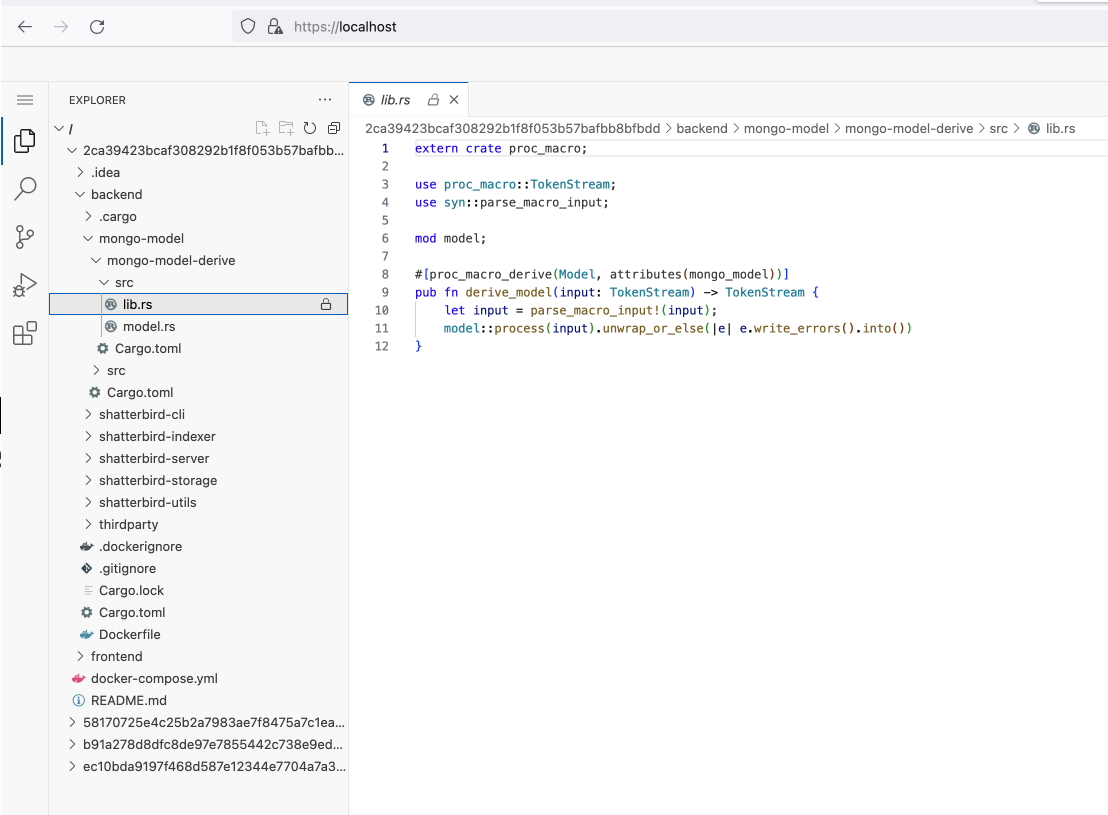
\includegraphics[width=\textwidth,height=0.5\textheight,keepaspectratio]{figures/intro.png}
    \caption{Скриншот пользовательского интерфейса, доступного по протоколу https}
\end{figure}

\section{Процесс индексирования}

Индексация репозитория разделяется на два этапа: загрузка объектов Git и загрузка данных результата индексации в формате LSIF. Оба этих этапа можно осуществлять с помощью программы \texttt{shatterbird-indexer}.

Во-первых, рассмотрим процесс загрузки объектов Git. Для загрузки объектов репозитория необходимо указать строку подключения к базе данных и путь к корню репозитория. Сам же процесс загрузки можно описать следующим алгоритмом:

\begin{enumerate}
    \item Найти текущий коммит в репозитории и проверить его наличие в базе данных. Если уже был загружен, то алгоритм можно завершить.
    \item Если у него есть родительские коммиты, то выполнить этот алгоритм рекурсивно, используя в качестве текущего коммита по очереди каждый из родительский. Можно не выполнять рекурсивно, если глубина загрузки истории уже больше, чем максимально указанная пользователем.
    \item Найти корневую директорию этого коммита и убедимся, что она не загружена в базу данных. Назовём её текущей.
    \item \label{git-upload-algo-dir-1} Для всех файлов в текущей директории проверить их наличие в базе данных. Если файл отсутствует, то загрузить его и все содержащиеся в нём строки. В этот момент возможно загрузить из базы данных предыдущие версии файла (из родительских коммитов) и переиспользовать ранее существовашие строки, чтобы сохранить построенные для них индексы.
    \item \label{git-upload-algo-dir-2} Для всех директорий в текущей директории также проверить наличие в базе данных. Если директория отсутствует, то выполнить рекурсивно пункты \ref{git-upload-algo-dir-1}-\ref{git-upload-algo-dir-2}, используя по очереди каждую ещё не загруженную директорию в качестве текущей.
    \item После того как корневая директория и все её потомки были загружены в базу данных, необходимо также загрузить объект коммита, включая в него ссылки на его родителей и ссылку на корневую директорию. Если какой-либо из родителей не был загружен в базу данных, то их нужно пропустить.
\end{enumerate}

В итоге в базе данных дублируются объекты Git-репозитория с использованием моделей, описанных в приложении \fullref{addendum:models}. А именно, используются объекты \texttt{Commit} для описания объектов коммитов и объекты \texttt{Node} для описания файлов и директорий.

Во-вторых, рассмотрим алгоритм загрузки графа LSIF в базу данных. Для этого на вход программе подается граф в виде списка JSON-строк: можно загрузить из файла, а можно прочитать из стандартного входа. Также необходимо в параметрах командной строки указать строку подключения к базе данных.

\begin{enumerate}
    \item Сначала необходимо загрузить граф из файла в память. При этом запоминаются все вершины графа, а для каждого также составляется список ребёр \textbf{исходящих} из него. Сразу дополнительно собирается список ссылок на те вершины, которые отражают документы (файлы).
    \item Затем для каждой вершины-документа из графа в Git-репозитории ищется соответствующей ей объект файла. Это позволяет сопоставить каждую вершины-документа с ранее загруженным в базу данных файловым объектом.
    \item Для каждой вершины типа «Range» ищется соответствующий ему файл, а в нём — нужная строка. Это необходимо, потому что файлы хранятся как массив строк, к которым и привязывается граф. Затем в базе данных подготавливается объект Range, содержащий идентификатор строки, начало и конец отрезка в ней, а также полный путь к этому файлу, начиная от корневой директории и заканчивая найденным файлом. Путь хранится как массив идентификаторов соответствующих объектов Node в базе данных.
    \item Наконец, запускается рекурсивный обход графа в глубину, начиная с каждой из вершин-документов. При этом все посещаемые вершины получают уникальный ObjectID (совместимый с MongoDB) и конвертируются в структуру, совместимую с хранимой в базу данных моделью данных. Аналогично обрабатываются ребра графа, но только после посещения всех вершин, которые связывает каждое отдельное ребро.
    \item Затем все эти объекты загружаются в базу данных.
\end{enumerate}

Для реализации этого алгоритма на языке Rust используется паттерн «Arena», который заключается в аллокации всех элементов графа (вершин и ребер) в одной структуре с единым временем жизни. Это позволяет легко гарантировать, что ребра, содержащие ссылки на вершины, будут все уничтожены одновременно с вершинами графа. Таким образом содержащиеся в ребрах ссылки никогда не будут висячими. Хотя такой подход и не позволяет освобождать память у отдельных объектов, но в данном случае этого и не требуется.

Благодаря использования итераторов и использования потокобезопасных коллекций, многие этапы алгоритма выполняются параллельно и используют все доступные потоки процессора.

\section{Инструмент для отладки}

Также во время работы над проектом был разработан вспомогательный инструмент для облегчения отладки и разработки системы. Он позволяет визуализировать граф, находящиеся в базе данных.

При запуске инструмента указывается идентификатор вершины графа, окрестности которого необходимо визуализировать. Затем, используя данные из базы данных, производится обход графа от этой вершины. Осуществляется поиск всех входящих рёбер и всех исходящих рёбер. Затем рекурсивно посещаются вершины по другую сторону кадждого ребра. Причем вершины типов Document и Moniker пропускаются, поскольку они связаны с большим количеством других вершин и значительно усложняют восприятие графа.

В процессе этого обхода каждое ребро и вершины записываются в формате dot для дальнейшей визуализации, причем начальная вершина дополнительно выделяется цветом, а все рёбра и вершины получают подписи с их типом. Дополнительно для вершин типа «Range» (то есть, указывающих на подстроки в файлах) добавляется подпись, содержащая эту подстроку и номер строки, в которой она содержится. Имя файла для таких вершин доступно при наведении курсора на вершину (при просмотре получившегося SVG файла).  После того как обход графа был завершен, полученный файл в формате dot преобразуется в SVG с использованием установленной на компьютере утилиты \texttt{neato}.

Важной особенностью утилиты является возможность выводить получившееся изображение прямо в терминал, с использованием специальных расширений (поддерживаются эмуляторы терминала iTerm2 и Kitty). При необходимости вывода на экран полученное SVG-изображение сперва преобразуется в растровое в формате PNG c помощью библиотеки resvg.

Примером работы программы является рис. \ref{fig:lsif-graph}.

\section{Описание контейнеров для запуска проекта}

Для облегчения запуска системы, используется система контейнеризации Docker и утилита docker-compose. Это позволяет обеспечить воспроизводимую сборку системы, а также позволяет описать все параметры конфигурации  и запуска в файлах, которые затем будут версионироваться и распространяться вместе со всем остальным кодом проекта.

Сборка серверной части описывается в Dockerfile, состоящим из этапа сборки и трех этапов, копирующих скомпилированные файлы для создания отдельных образов под разные программы: cli, indexer и server. Такой подход позволяет одновременно выполнить достаточно трудоемкое скачивание зависимостей и компиляцию только однажды при сборке первого этапа и при этом не включать исходные коды и промежуточные артефакты сборки вместе с конечными образами контейнеров — те содержат только единственный бинарный файл с соответствующим образу программой.

Сборка клиентской части также является многоэтапной: на первом этапе скачиваются все зависимости и собираются файлы сайта, а второй этап копирует получившийся результат в финальный образ, а также включает в него веб-сервер Caddy и его конфигурацию.

Наконец, все эти образы координируются с помощью файла docker-compose.yml, который позволяет при сборке указывать тег для каждого собранного образа, а также описывает конфигурацию запуска всей системы. Система состоит из трёх контейнеров: бекенд, база данных и фронтенд. При этом доступ к базе данных часто нужен из вспомогательных контейнеров при индексации, а фронтенд взаимодействует только с бекендом. Поэтому в рамках docker-compose описываются две сети: front и back. В первую сеть включен только фронтенд и бекенд, а во вторую — только бекенд и база данных. При этом предполагается, что в сети back также будут запускаться короткоживущие контейнеры при загрузке новых индексов.

Также docker-compose.yml описывает запуск контейнера с базой данных MongoDB. Для обеспечения персистентности данных, объявляется и используются специальный том «mongo-data», в котором хранятся данные. Аналогично при помощи тома обеспечивается персистентность для обратного прокси — тот сохраняет на диск информацию о полученных TLS-сертифкатов и эти данные должны сохраняться между перезапусками контейнера.

Для того, чтобы дать вспомогательным образам indexer и cli имена, они также упоминаются в файле docker-compose.yml, но отмечены для использования только в профиле сборки. Таким образом при запуске системы с помощью обычного профиля они не будут каким-либо образом использоваться, но участвуют в сборке и получают в её процессе имена.

Наконец, чтобы облегчить пользователю развертывание системы, файл конфигурации обратного прокси Caddy устроен так, что позволяет указать домен с помощью переменной окружения. Таким образом, при развертывании системы достаточно только указать в docker-compose.yml используемый домен (например, «\texttt{example.org}»), чтобы веб-сервер автоматически обрабатывал запросы только для этого домена и получил для него TLS-сертификат.

\section{Документирование исходного кода и юнит-тесты}

Для серверной части используются встроенные в стандартную поставку языка инструменты для документирования и тестирования. Это позволяет с использованием команды «\texttt{cargo doc}» автоматически сгенерировать документацию ко всем типам, а с помощью команды «\texttt{cargo test}» запустить все юнит-тесты. При этом код юнит-тестов не включен в релизную сборку и не увеличивает размер бинарного файла, не ухудшает быстродействие программы и не увеличивает время компиляции. Эта особенность тестов и простота их запуска также позволяет во время запуска тестов автоматически обновлять сгенерированные описания моделей данных на языке Typescript для их дальнейшего использования в коде клиентской части.

Код клиентской части, написанный на языке Typescript, не применяет никаких инструментов для документации и юнит-тестирования, поскольку объем кода достаточно небольшой, а юнит-тестирование расширения для Visual Studio Code достаточно трудоемко.

\section{Выводы по главе}

В этой главе были подробны описаны детали реализации системы: общая архитектура и структура проекта, приведено описание всех лежащих в её основе отдельных программ. Приводится подробное описание алгоритма индексирования и устройство работы пользовательского интерфейса, а также описаны особенности эффективного данных. Наконец, описывается взаимодействие отдельных компонентов друг с другом и приводится использование Docker для сборки и запуска проекта.

\clearpage
